\section{Data Center Telkom}
\tab Teknologi cloud computing di Indonesia telah berjalan, dimana PT. Telekomunikasi Indonesia atau PT. Telkom telah bekerja sama dengan Microsoft dalam hal teknologi cloud computing. Layanan ini dapat membuat perusahaan dengan cepat dan mudah meningkatkan kapasitas penyimpanan, karena didapat secara virtual. Solusi yang dikembangkan oleh PT.Telkom dan Microsoft hadir dalam bentuk Microsoft Windows Exchange dan Office Communications Server Hosted dimana merupakan salah satu jalan untuk membantu bisnis di Indonesia mengadopsi teknologi cloud computing dengan biaya relatif murah. Pihak Microsoft dan PT. Telkom sepakat untuk mengembangkan bisnis cloud  computing  mulai  dari Infrastructure as a Service (IAAS), Platforms as a Service (PAAS) dan Software as a Service (SAAS) yang dikirimmelalui cloud yang aman.\\
Layanan ini mampu memberikan solusi komprehensif bagi bisnis dan insdustri  serta memberikan percepatan dalamnegeri ini pada era teknologi  cloud computing.\\
Ada  beberapa  paket  yang  ditawarkan  oleh  PT.  Telkom  dengan  teknologi   cloud  computing
diantaranya:
\begin{enumerate}
\item Paket Communication dan  Collaboration.\\
Broadband + Exchange + OCS, sebuah bentuk SaaS yang memberikan fitur teknologi microsoft united communication tanpa harus di install. Hosted OCS menawarkan  :  instant messaging dan presence, email dan united messaging, peer-to-peer voice dan video, desktop sharing di microsoft office, communication 207 R2, web-based IM, email, presence dan desktop sharing.
\item Paket  Virtualized Server\\
Broadband + virtual Dedicated Server, sebuah bentuk IaaS. Teknologi VPS (Virtual Private Servers), memungkinkan sebuah perusahaan dapat berbagi  biaya  server dengan pelanggan yang lain dengan tetap memegang kendali penuh terhadap aplikasi mereka. VPS berjalan pada web server dan memberikan akses dengan privasi  penuh dan bandwidth yang terjamin, CPU dan ruang disk.
\end{enumerate}
Pada dasarnya telkom memberikan sistem online data dimana solusi untuk sebuah perusahaan untuk mengelola data, khususnya data konsumen atau calon konsumen, teknologi ini memberikan layanan pengadaan yang bisa memberikan sistem data dan teknologi yang saling terintergrasi, reliable dan update.\\
Pada layanan ini akan dikombinasikan keseluruhan layanan yang diberikan. Produk ini dapat menjamin kegiatan bisnis yang menjamin status data selalu terupdate sepanjang tahun. Dipadu dengan kemampuan SDM yang berpengalaman dalam pengelolaan database, juga system dan data-data yang selalu terjaga dalam kondisi optimal sehingga dapat digunakan untuk berbagai kebutuhan. Hal tersebut diintegrasikan dengan kompetensi utama lainnya dari PT. Infomedia Nusantara yaitu berupa Contact Center Solutions yang dapat memberikan berbagai alternative pengadaan proses inbound/outbound call perusahaan dan juga dengan layanan Produk Konten Infomedia, yang dapat memberikan solusi lain dalam hal pengakuisisian kelengkapan data bagi kebutuhan perusahaan dan layanan outbound service berupa sms dan direct mail.\\
\begin{center}
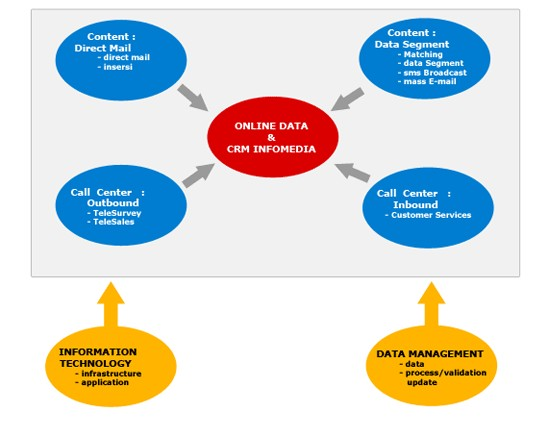
\includegraphics[scale=1]{gambar411.jpg}\\
Gambar 4.1.1  Arsitektur online data
\end{center} 
Layanan ini disediakan dengan menggunakan system online yang mana menghubungkan system data yang digunakan khusus bagi pelanggan dengan database yang terdapat di Infomedia. Dengan data processing system yang online, maka akan memberi kemudahan kepada customer untuk dapat menerima data-data sesuai dengan kondisi data yang ada di Infomedia.\\
\begin{center}
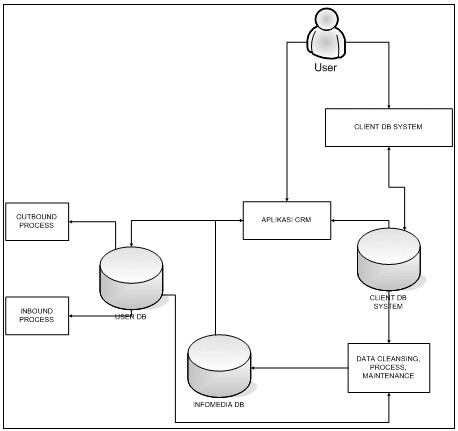
\includegraphics[scale=1]{gambar412.jpg}\\
Gambar 4.1.2  Sistem online data
\end{center}
Tujuh alasan utama menggunakan sistem secara online dimana sistem tersebut  di implementasi kan di sekolahan oleh pihak Telkom,  diantaranya :
\begin{enumerate}
\item Sistemnya serba Online dan Real-Time dapat diakses setiap saat dari mana saja\\
SIAP Online dibangun 100\% berbasis teknologi web versi 2.0 untuk dapat  diakses secara online 24 jam setiap saat dan dan dari mana saja selama Anda memiliki koneksi ke Internet. Setiap ada pengubahan data secara online, sistem SIAP Online akan memprosesnya secara langsung dalam waktu nyata (real time) untuk menjamin kenyamanan dan kesahihan setiap pengubahan (edit) data yang Anda lakukan.
\item Biaya terjangkau dan minim investasi/modal\\
Layanan SIAP Online tidak memerlukan lisensi perangkat lunak (licenced software) khusus sebagaimana produk lainnya. Anda juga tidak memerlukan investasi/modal perangkat server khusus yang terpasang lokal di sekolah atau dinas untuk mengoperasikan sistem SIAP Online. Yang Anda perlukan hanyalah sebuah web  browser di PC/ Laptop Anda yang terkoneksi ke Internet.\\
Semua perangkat utama seperti: server-server, sistem aplikasi, backup data, keamanan data hingga pemeliharaan sistemnya merupakan tanggung jawab TELKOM sebagai penyedia layanan. Dengan demikian layanan SIAP Online akan menurunkan total  biaya penggunaannya untuk Anda, institusi Anda (sekolah dan dinas). Institusi Anda juga tidak perlu melakukan investasi/modal awal yang sangat mahal. Dengan ini  maka  Institusi Anda terhindar dari resiko kerugian investasi/ modal.\\
TELKOM sangat sarankan agar Anda tidak begitu saja mudah percaya dengan layanan SIAP Online kami. Untuk itu kami memberikan kesempatan bagi Anda untuk mempelajarinya secara menyeluruh, kami menyediakan akses versi demo dan versi ujicoba (trial) sebelum Anda benar-benar yakin untuk berlangganan SIAP Online versi komersial.
\item Aplikasinya nyaman dan lengkap sesuai  kebutuhan setiap pengguna\\
SIAP Online tidak hanya menyediakan aplikasi untuk pengelolaan data pendidikan saja seperti: data siswa, data guru, data orangtua/wali siswa, kelas, jadwal, kurikulum mata pelajaran. Beragam aplikasi kami sediakan untuk mendukung terciptanya suasana akademis di lingkungan sekolah dan dinas seperti: sms, email, web sekolah,  pustaka,  dan lain-lain.Untuk kenyamanan Anda mengakses beragam layanan tersebut, SIAP Online menerapkan sistem satu login multi layanan, Anda hanya cukup mengingat satu nama pengguna (username) dan kata kunci (password) untuk mengakses layanan- layanan yang kami sediakan.\\
Kami selalu berupaya memberikan layanan terbaik untuk Anda. Para insinyur pengembang kami akan selalu mengembangkan layanan SIAP Online untuk mengakomodir kebutuhan setiap penggunanya dari waktu ke waktu.\\
Untuk itu kami sangat berharap selalu mendapatkan saran dan masukan dari Anda dalam upaya melengkapi dan menyempurnakan fitur-fitur sistem menyesuaikan dengan kebutuhan Anda. Para insinyur pengembang kami akan berupaya merilis aplikasi/fitur terbaru sesuai masukan dari Anda setiap waktu di SIAP Online dengan nyaman tanpa perlu ada instalasi ataupun kerumitan upgrade/update di sisi Anda sebagai pengguna  aktif SIAP Online. Kenyamanan Anda sangat berarti bagi  kami.
\item Skalabilitas tinggi, aman, handal,  mudah dan cepat diimplementasikan\\
Sistem SIAP Online dirancang menggunakan teknologi berbasis Web versi 2.0 dengan didukung lingkungan awan komputasi (cloud computing) yang handal dan platform yang berarsitektur multi pelanggan (multi-tenant architecture). Anda tidak perlu mengalami kerumitan pengalaman terhadap pengelolaan sistem sendiri, semua hal terkait dengan pengorganisasian, pengembangan dan pemeliharaan sistem dibelakang (backend) layanan SIAP Online merupakan tanggung jawab TELKOM sebagai penyedia layanan.Skalabilitas dan keamanan data pada layanan SIAP Online akan selalu terjaga, kami tidak membatasi jumlah data dan pengguna selama sekolah dan dinas menjadi pelanggan SIAP Online. Data Anda akan selalu disimpan dan dicadangkan (backup) di lingkungan awan komputasi  kami yang tersebar dibeberapa lokasi.\\
Dengan dukungan sistem dibelakang (backend) SIAP Online yang handal, kami juga menyediakan kemudahan bagi insitusi Anda (sekolah dan dinas) untuk menjadi pelanggan SIAP Online, hanya dengan 3 (tiga) langkah mudah, institusi Anda sudah dapat  berlangganan SIAP Online.
\item Terintegrasi  dengan beragamfasilitas dan layanan online lainnya\\
Sebagai bagian dari komitmen kami untuk dapat menyediakan layanan pendidikan yang penuh fitur dan terintegrasi satu dengan yang lain. Kerangka kerja (framework) sistem SIAP Online dirancang terbuka untuk interkoneksi dengan aplikasi, fasilitas dan layanan online lainnya. Baik aplikasi yang dikembangkan oleh TELKOM secara langsung atau sistem yang dikembangkan pihak mitra kerja TELKOM atau yang disediakan oleh pihak ketiga di Internet.Contoh aplikasi yang terintegrasi dengan SIAP Online antara  lain adalah SMS gateway TELKOM Flexi, autentifikasi Speedy SchoolNet, TELKOM iVAS, Flexi Cash, host to host sistempembayaran perbankan, dan berbagai  sistem lainnya.\\
Kami siap membantu secara teknis untuk mengaktifkan layanan GoogleApps bagi institusi Anda sesuai syarat dan ketentuan yang berlaku. Silahkan pelajari prosedur pengaktifan GoogleApps Anda.\\
Melalui integrasi dengan berbagai fasilitas dan layanan inline ini, TELKOM berharap memberikan kemudahan bagi  pengguna SIAP Online
\item Satu login pengguna untuk akses seluruh layanan yang tersedia\\
Seluruh proses otentifikasi, otorisasi dan identifikasi para pengguna (user) pada sistem SIAP Online dirancang sedemikian rupa untuk mendukung upaya satu login multi layanan dengan kerangka kerja single sign on system. Mekanisme ini untuk menambah kenyamanan bagi seluruh pengguna pelanggan SIAP Online dalam mengoperasikan akses ke berbagai layanan online yang kami sediakan dengan hanya mengingat satu login (username and password) saja.\\
Pengaturan hak akses setiap individu pengguna dapat dilakukan secara mandiri oleh admin sekolah atau dinas yang telah berlangganan SIAP Online. Bagi para admin sekolah dan dinas dapat memonitor dan mengendalikan hak akses  para siswa,  guru, dan orangtua siswa dengan mudah dan nyaman.
\item Fleksibel  dan uptodate mengikuti perkembangan aturan pendidikan di Indonesia\\
Pengembangan sistem akan selalu dijaga uptodate oleh kami tidak hanya terbatas pada aplikasi perangkat lunak atau sistem dibelakang (backend). Anda tidak perlu kuatir memodifikasi sistem atau aplikasi di SIAP Online jika diperlukan untuk menyesuaikan dengan aturan-aturan pendidikan yang diberlakukan secara nasional. Percayakan dan serahkan kepada insinyur pengembang kami yang akan membantu Anda dalam melakukan update sistem menyesuaikan dengan aturan-aturan yang berlaku di dunia pendidikan Indonesia dengan konsisten.SIAP Online telah kami rancang untuk turut mendukung kebijakan serta program-program dari Departemen Pendidikan Nasional (Depdiknas). Saat ini sangat kami rekomendasikan bagi para pelanggan SIAP Online untuk basis data siswa dan sekolah menggunakan layanan Dapodik (Data Pokok Pendidikan) yang disediakan oleh Depdiknas.\\
Walaupun demikian, kami telah mengembangkan sistem yang mampu menghadapi berbagai kebutuhan lokal. Beberapa pilihan katalog aturan yang flexibel untuk berbagai pilihan sesuai regualasi lokal  yang berlaku berbeda-beda untuk setiap Dinas Pendidikan.
\end{enumerate}
\section{Virtualisasi  dan integrated network pada PT. Kian Ho Indonesia}
\tab PT. Kian Ho Indonesia merupakan perusahaan distributor bearing resmi di Indonesia dan  bagian subsidiary dari Kian Ho Bearing Pte Ltd yang berkantor pusat di Singapore. Kian Ho Bearing Pte Ltd adalah salah satu perusahaan distributor resmi bearing yang go public memiliki beberapa subsidiary di 7 negara dan banyak cabang yang tersebar di beberapa negara lain.\\
Sebagai subsidiary dari Kian Ho Bearing Pte Ltd, PT Kian Ho Indonesia menerapkan beberapa sistem informasi dan sistem network yang saling terintegrasi untuk menunjang operasional sehari-hari. Beberapa sistem yang diimplementasikan :
\begin{itemize}
\item SCMNavision
\item LPO dan Stockcard web
\item MRTG( Multi Router Traffic Grapher  )
\item Helpdesk dan IT manajemen system
\item VMware
\end{itemize}
SCM Navision merupakan sistem supply chain management yang diimplementasikan untuk menunjang operasional distribusi bearing dari Singapore ke Indonesia, yang nantinya bearing tersebut akan didistribusikan di seluruh area Indonesia ke beberapa supplier baik OEM Indonesia maupun retail bearing di seluruh Indonesia. SCM Navision adalah bagian internal sistemTI dari Kian Ho Bearing Pte Ltd Singapore.\\
LPO dan Stockcard web merupakan sistem berbasis web yang diimplementasikan untuk menunjang operasional pembelian bearing di Indonesia ( antar local distributor bearing di Indonesia ) dan sistem stockcard yang berfungsi mengintegrasikan seluruh asset inventory dari perusahaan PT Kian Ho Indonesia.\\
MRTG merupakan sistem monitoring network penunjang operasional. Seperti MRTG pada umumnya sistem ini untuk memonitor segala aktifitas traffic yang terjadi baik internal network maupun koneksi internet.\\
Helpdesk sistem merupakan sistem helpdesk untuk memonitor aktifitas keluhan karyawan terhadap performance TI. Sedangkan IT manajemen system merupakan sistem integrasi  seluruh perangkat TI berbasis network, aktifitas seluruh asset TI ( workstation komputer, server, printer, router, switch dan PABX ) di kelola dan di monitor melalui satu software atau aplikasi.
\subsection{Integrasi  antar sistem}
\tab Manajemen PT Kian Ho Indonesia menyadari beragamnya aplikasi yang ada dan memperhatikan sisi efisiensi operasional TI. Maka diperlukan satu software yang dapat mengakomodasi dan menjalankan seluruh aplikasi  penunjang serta menghasilkan  infrastruktur TI terkendali.\\
Software tersebut adalah VMware yang merupakan produk  software virtualisasi  dari  vmware inc. Software vmware ini diimplementasikan pada satu server blade, dan menjalankan beberapa aplikasi penunjang operasional dalam sistem operasi yang berbeda – beda sesuai kebutuhan aplikasi tersebut.\\
Sistem operasi yang digunakan adalah linux ( Ubuntu Server ) dan Windows Server. Aplikasi penunjang seperti LPO berbasis web, stockcard berbasis web, sistem helpdesk berbasis web diimplementasikan dalam windows XP, untuk aplikasi SCM Navision lebih bersifat client side dan digunakan melalui  mekanisme RDC ( Remote desktop connection ).\\
Aplikasi penunjang yang lain seperti IT management system dan database dari masing  – masing aplikasi tersebut diimplementasikan ke dalam sistem operasi linux. VMware diimplementasikan dalam sistemoperasi Windows Server Enterprise 2003. Seperti yang terlihat pada gambar 4.2.1.
\begin{center}
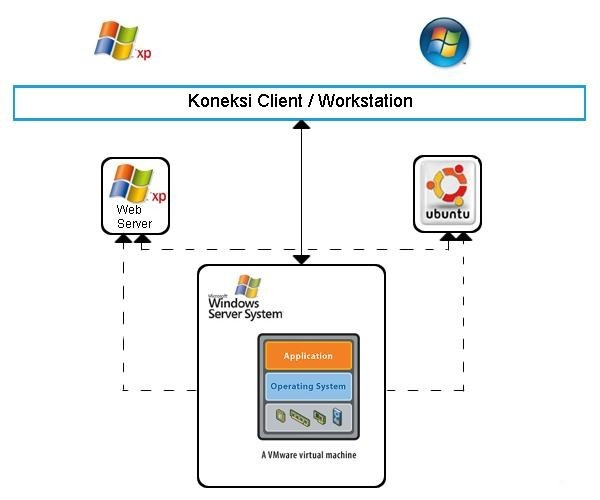
\includegraphics[scale=1]{gambar421.jpg} \\
Gambar 4.2.1 VMware pada Windows Server Enterprise 2003
\end{center}
Topologi jaringan yang terbentuk secara global, seperti yang terlihat pada gambar 4.2.2
\begin{center}
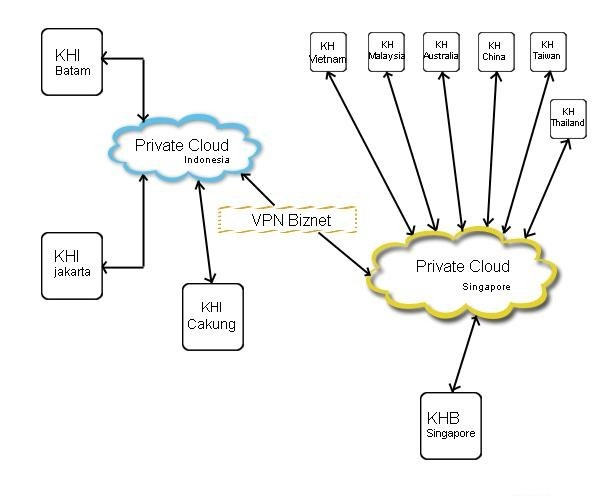
\includegraphics[scale=0.71]{gambar422.jpg} \\
Gambar 4.2.2 Topologi Jaringan Global
\end{center}
Server blade yang menjadi server utama berpusat di Jakarta dan menjadi data center bagi operasional KHI ( Kian Ho Indonesia ). Sedangkan aplikasi penunjang berada dalam mesin virtual, seperti yang terlihat pada gambar 4.2.3
\begin{center}
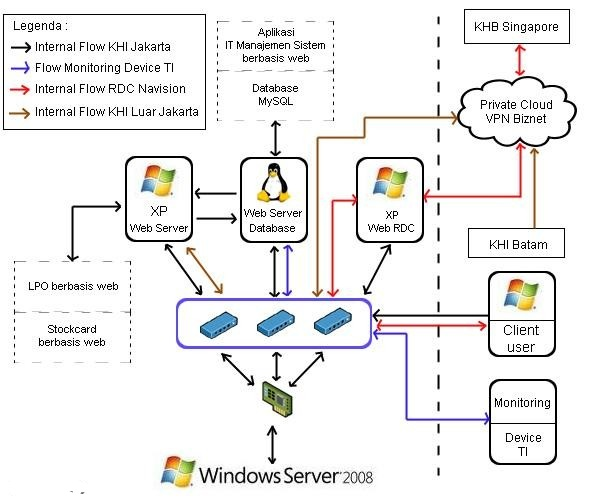
\includegraphics[scale=0.71]{gambar423.jpg} \\
Gambar 4.2.3 Aplikasi Penunjang dalam VM
\end{center}
Windows Server 2008 diimplementasikan ke server blade, dan terbagi dalam tiga mesin virtual yaitu dua buah mesin virtual dengan sistem operasi windows XP, dan satu buah mesin virtual berbasis linux.\\
\tab KHI ( PT Kian Ho Indonesia ) sebagai subsidiary KHB ( Kian Ho Bearing Pte Ltd ) Singapore memiliki autorisasi untuk menerapkan TI policy ( aturan ) secara mandiri untuk diterapkan dalaminfrastruktur  TI di Indonesia.\\
Infrastruktur TI di KHB Singapore menerapkan SCMNavision untuk menunjang operasionalnya, sesuai policy ( aturan ) TI KHB Singapore, semua subsidiary dari KHB diwajibkan untuk menggunakan SCM Navision melalui protocol RDC ( remote desktop connection ) dan koneksi yang terjadi harus melalui VPN internet dengan enkripsi IPSec.\\
Semua pemesanan dan pengiriman barang baik dari Singapore ke Indonesia maupun dari Indonesia ke Singapore melalui software atau aplikasi SCMNavision.\\
\tab Manajemen KHI menyadari pentingnya SCM Navision dalam menunjang  operasional serta menyadari kepentingan internal KHI yang bersifat confidential ( rahasia untuk  KHB  ), maka TI manajemen KHI menyerahkan tanggung jawab koneksi internet ( VPN dan implementasi keamanan transaksi ) kepada provider ISP yaitu  Biznet.\\
Untuk kepentingan internal KHI maka dibuat dua mesin virtual dengan sistem operasi yang sejenis yaitu windows XP ( gambar 4.2.3 ). Mesin virtual pertama menangani dan bertanggung jawab   terhadap   semua   aktifitas  user   ketika  mengakses   web  service,   Pada  mesin  virtual pertama hanya aplikasi yang diimplementasi, tetapi database terkoneksi pada mesin virtual berbasis linux. Aliran alur jaringan dapat dilihat pada gambar 4.2.3 dengan anak  panah berwarna hitam($\rightarrow$).\\
Aplikasi yang diimplementasikan pada mesin virtual pertama adalah LPO berbasis web, dan stockcard berbasis web. Dalam perencanaan TI di kemudian hari skalabilitas dari aplikasi LPO dan stockcard akan ditingkatkan dimana saat ini skalabilitasnya terkoneksi ke BB dan ke email.\\
Aplikasi pada mesin virtual pertama, menggunakan php berbasis framework dengan web servernya adalah Abyss Web Server.
Ketika user dari KHI batam dan KHI cakung terkoneksi ke aplikasi LPO dan stockcard melalui internet, maka server blade yang memiliki IP public dengan kemampuan virtual manajemen sistem vmware, akan menjalankan dan meneruskan request ini ke mesin  virtual  pertama dimana aplikasi LPO dan stockcard diimplementasikan. Aliran alur jaringan dapat dilihat pada gambar 4.2.3 dengan anak panah berwarna coklat (\textcolor{brown}{$\rightarrow$}).\\
/tab Mesin virtual kedua menjadi pusat data dari semua aplikasi internal KHI, database yang digunakan adalah mysql. Aplikasi IT manajemen sistem berfungsi sebagai aplikasi  realtime  yang  memonitor semua device atau peralatan TI yang dijadikan sebagai asset IT.\\
Secara berkala aplikasi IT manajemen sistem akan mengecek kondisi dan status peralatan TI KHI yang berbasis network, hal ini dilakukan dengan tujuan pengendalian atau kontroling terhadap peralatan tersebut, sehingga setiap problem dari peralatan  TI  KHI  dapat  terdeteksi dan mendapatkan alert sistemkepada teamhelpdesk TI KHI. Seperti  yang terlihat pada gambar 4.2.3 dengan anak panah berwarna biru (\textcolor{blue}{$\rightarrow$}).\\
/tab Mesin virtual ketiga merupakan windows XP yang difungsikan sebagai workstation atau komputer client dengan tujuan untuk menyatukan koneksi VPN, dan melakukan remote desktop connection ( RDC ) untuk pemakaian SCM Navision di private cloudnya LHB Singapore
\begin{center}
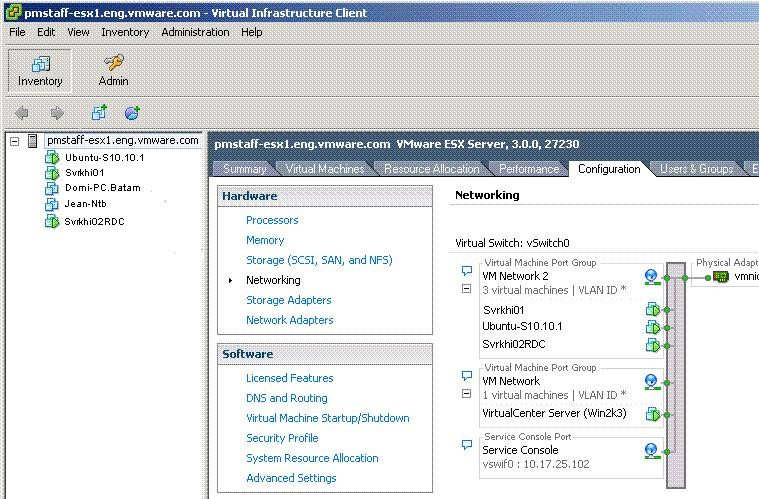
\includegraphics[scale=0.71]{gambar424.jpg} \\
Gambar 4.2.4 interface virtual management  system VMware
\end{center}
\begin{center}
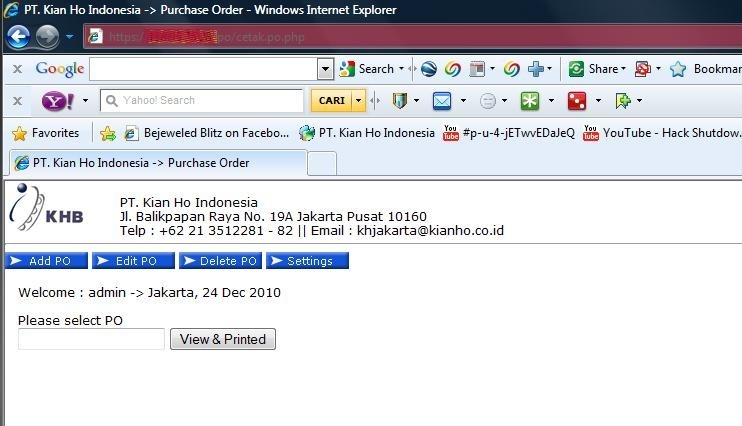
\includegraphics[scale=0.71]{gambar425.jpg} \\
Gambar 4.2.5 aplikasi LPO berbasis web
\end{center}
Gambar 4.2.5 merupakan aplikasi LPO berbasis web yang dapat diakses melalui internet dan untuk keperluan internal. Pengguna memerlukan userid dan password yang setiap bulan akan berganti. Aplikasi ini juga memiliki alert sistem untuk menyetujui transaksi yang terjadi, dan alert tersebut terkirim ke blackberry dan email sistem
\begin{center}
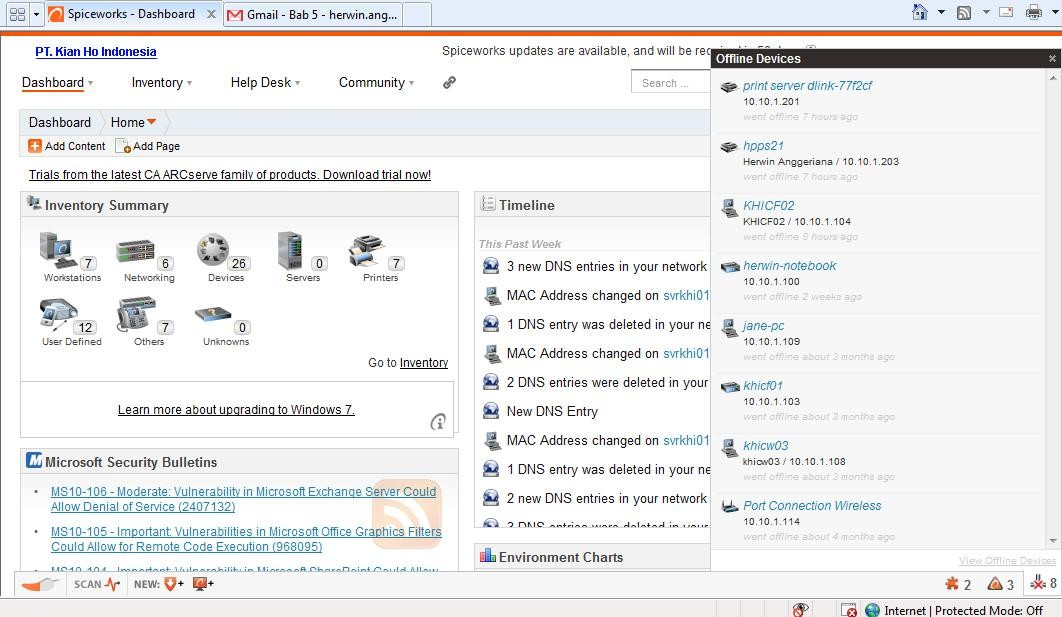
\includegraphics[scale=0.5]{gambar426.jpg} \\
Gambar 4.2.6 aplikasi IT management.
\end{center}
Gambar 4.2.6 merupakan aplikasi IT management system, yang merupakan aplikasi berbasis web dapat diakses melalui internet, dibangun dengan framework php. API yang diterapkan dalamaplikasi ini lebih difokuskan kepada fungsi  monitoring peralatan TI di KHI.
\begin{center}
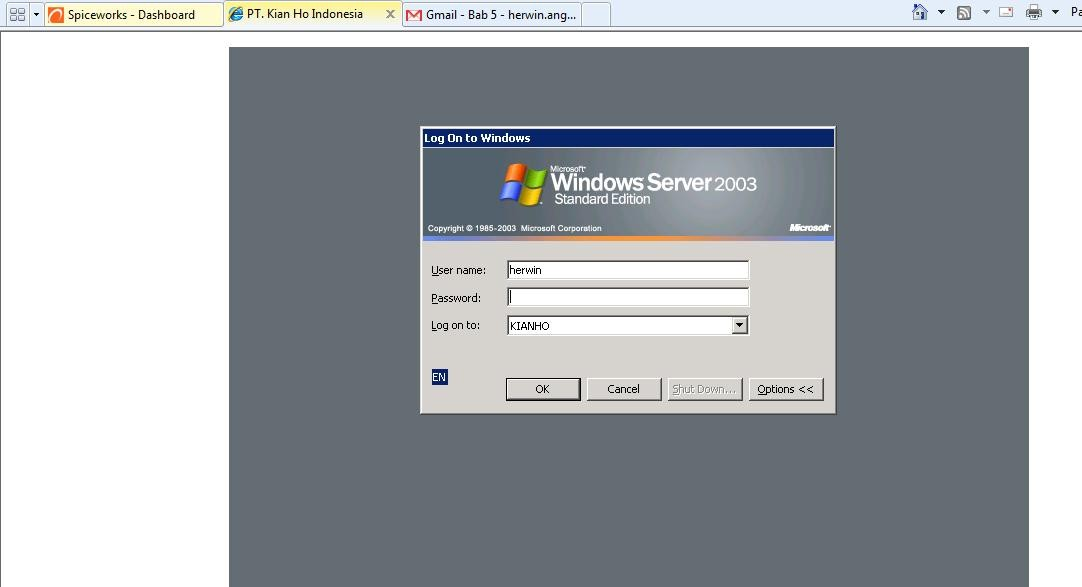
\includegraphics[scale=0.5]{gambar427.jpg} \\
Gambar 4.2.7 remote desktop connection berbasis web.
\end{center}
Gambar 4.2.7 merupakan remote desktop connection berbasis web, diimplementasikan dalam mesin virtual ketiga dengan sistem operasinya windows XP, ketika user  mengakses  mesin virtual ketiga melalui koneksi internet, maka secara automatis mesin virtual ketiga  akan terkoneksi dengan server KHB Singapore.  Aplikasi ini juga menggunakan platform API.\\
Jaringan pada mesin virtual ketiga ini didukung dengan private cloud melalui koneksi internet berbasis VPN IPSec yang disupply oleh provider Biznet.
\begin{center}
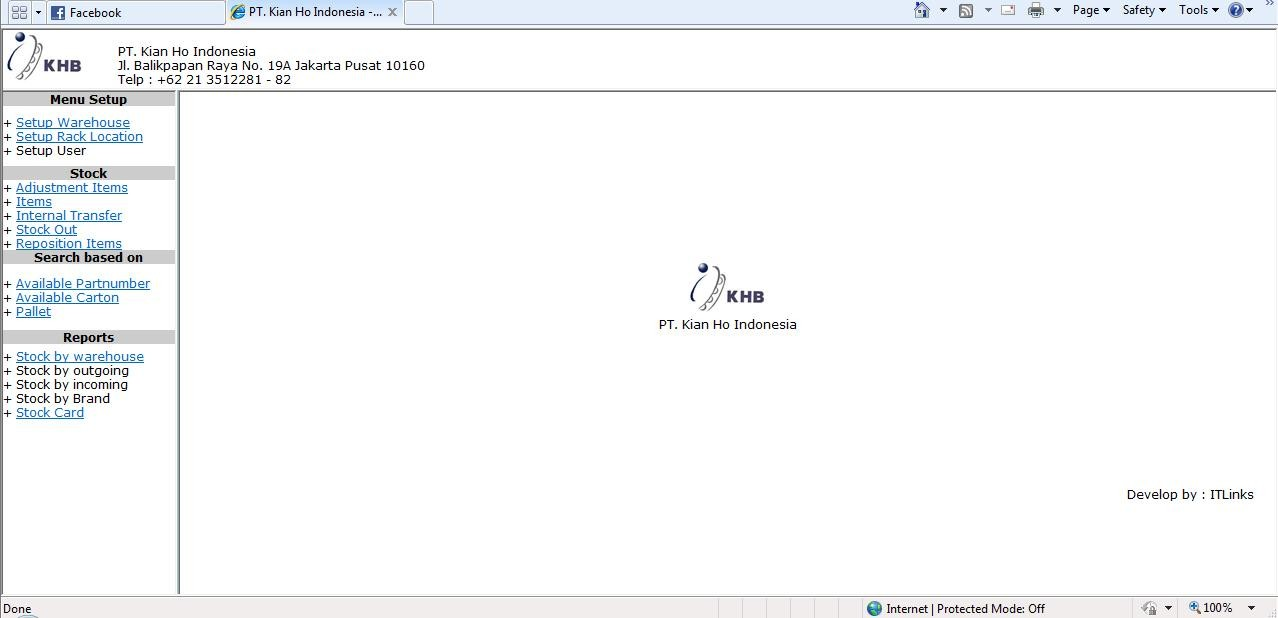
\includegraphics[scale=0.5]{gambar428.jpg} \\
Gambar 4.2.8 aplikasi stockcard berbasis web.
\end{center}
Gambar 4.2.8 merupakan aplikasi stockcard berbasis web yang  diimplementasikan  dalam  mesin virtual pertama, dengan database yang berada di mesin virtual kedua dengan sistem operasi linux.